\begin{figure}[]
\centering
\begin{subfigure}{.45\textwidth}
  \centering
  \begin{tikzpicture}[line width=2pt]
    \coordinate (m) at (2.25,-5);
    \coordinate (o) at (0,0);
    %
	\fill [pattern = north east lines] (-3.5,0) rectangle (3.5,0.5);
    %
    \draw (-3.5,0) to (3.5,0);
    \draw (o) to (m);
	\draw (1.2,-2.5) node[anchor=west]{\LARGE $l$};
    %
    \fill (m) circle (3.5pt);
    \draw (o) node[anchor=center]{\huge $\boldsymbol{\times}$};
    %
    \draw[-{Stealth[length=4mm, width=2.5mm]}] (-3,-2) to (-1.75,-2);
	\draw[-{Stealth[length=4mm, width=2.5mm]}] (-3,-2) to (-3,-0.75);
	\draw (-2.4,-1.4) node[anchor=center]{\Large $\boldsymbol{\bigodot}$};
	%
	\draw (-2.5,-2) node[anchor=north]{\LARGE $\vu{x}$};
	\draw (-3,-1.5) node[anchor=east]{\LARGE $\vu{y}$};
	\draw (-2.25,-1.35) node[anchor=west]{\LARGE $\vu{z}$};
	%
    \draw[dashed, line width=1pt] (o) to (0,-6.5);
    \draw[dashed, line width=1pt] (0,-5) to (m);
	\draw (1.125,-5) node[anchor=north]{\LARGE $x$};
	\draw (0,-2.5) node[anchor=east]{\LARGE $y$};
	%
	\draw [domain=-90:-65.77, line width=1.5pt] plot ({cos(\x)}, {sin(\x)});
	\draw (0.23,-1.25) node[anchor=center]{\LARGE $\phi$};
	%
	\draw[-{Stealth[length=4mm, width=2.5mm]}] (m) -- ++(24.23:1.25cm);
	\draw[-{Stealth[length=4mm, width=2.5mm]}] (m) -- ++(-65.77:1.25cm);
 	\draw (2.2,-5.5) node[anchor=center]{\LARGE $\vu{r}$};
 	\draw (3.1,-5.05) node[anchor=center]{\LARGE $\vu*{\phi}$};
 	%
 	\draw[-{Stealth[length=3mm, width=2mm]}, line width=1.5pt]
 	    (2.9,-3.85) node[anchor = west]{\LARGE $m$} [bend right=25] to (2.275,-4.85);
 	%
 	\draw[-{Stealth[length=3mm, width=2mm]}, line width=1.5pt]
 	    (-0.9,-0.65) node[anchor = east]{\LARGE $\mathcal{O}$} [bend right=25] to (-0.1,-0.2);
  \end{tikzpicture}
  %
%   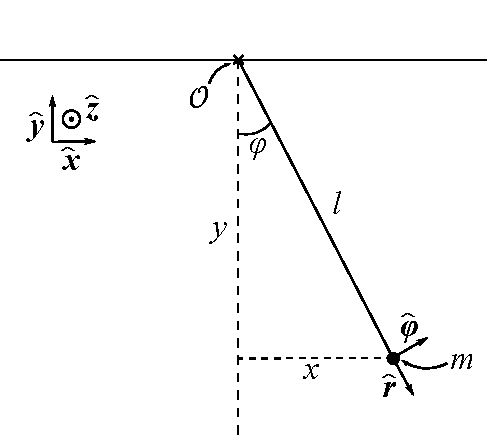
\includegraphics[width=\linewidth]{figurer/Pendul.pdf}
\caption{Skitsering af pendul med massen $m$ og længden $l$. Enhedsvektorerne til et kartesisk og et cylindrisk polært koordinatsystem er indtegnet.}
\label{mek:fig:Pendul}
\end{subfigure}
\hspace{5mm}
\begin{subfigure}{.45\textwidth}
  \centering
  \begin{tikzpicture}[line width=2pt]
    \coordinate (m) at (2.25,-5);
    \coordinate (o) at (0,0);
    %
	\fill [pattern = north east lines] (-3.5,0) rectangle (3.5,0.5);
    %
    \draw (-3.5,0) to (3.5,0);
    \draw (o) to (m);
	\draw (1.2,-2.5) node[anchor=west]{\LARGE $l$};
    %
    \fill (m) circle (3.5pt);
    \draw (o) node[anchor=center]{\huge $\boldsymbol{\times}$};
    %
    \draw[-{Stealth[length=4mm, width=2.5mm]}] (-3,-2) to (-1.75,-2);
	\draw[-{Stealth[length=4mm, width=2.5mm]}] (-3,-2) to (-3,-0.75);
	\draw (-2.4,-1.4) node[anchor=center]{\Large $\boldsymbol{\bigodot}$};
	%
	\draw (-2.5,-2) node[anchor=north]{\LARGE $\vu{x}$};
	\draw (-3,-1.5) node[anchor=east]{\LARGE $\vu{y}$};
	\draw (-2.2,-1.35) node[anchor=west]{\LARGE $\vu{z}$};
	%
    \draw[dashed, line width=1pt] (o) to (0,-6.5);
    \draw[dashed, line width=1pt] (0,-5) to (m);
	\draw (1.125,-5) node[anchor=north]{\LARGE $x$};
	\draw (0,-2.5) node[anchor=east]{\LARGE $y$};
	%
	\draw [domain=-90:-65.77, line width=1.5pt] plot ({cos(\x)}, {sin(\x)});
	\draw (0.23,-1.25) node[anchor=center]{\LARGE $\phi$};
	%
	\draw[-{Stealth[length=4mm, width=2.5mm]}] (m) -- ++(114.23:1.35cm);
	\draw[-{Stealth[length=4mm, width=2.5mm]}] (m) -- ++(-90:1.35cm);
 	\draw (2.6,-5.5) node[anchor=center]{\LARGE $\va{w}$};
 	\draw (1.45,-4.3) node[anchor=center]{\LARGE $\va{T}$};
 	%
 	\draw[-{Stealth[length=3mm, width=2mm]}, line width=1.5pt]
 	    (2.9,-3.85) node[anchor = west]{\LARGE $m$} [bend right=25] to (2.275,-4.85);
 	%
 	\draw[-{Stealth[length=3mm, width=2mm]}, line width=1.5pt]
 	    (-0.9,-0.65) node[anchor = east]{\LARGE $\mathcal{O}$} [bend right=25] to (-0.1,-0.2);
  \end{tikzpicture}
  %
%   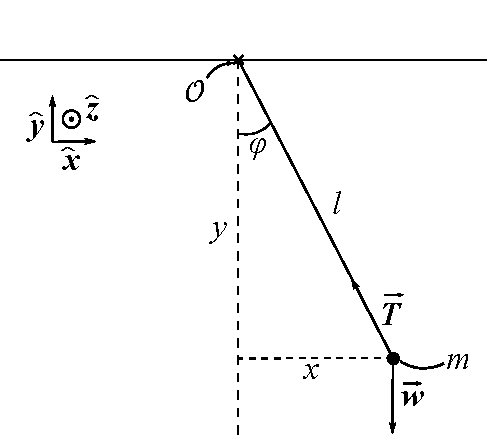
\includegraphics[width=\linewidth]{figurer/PendulKraft.pdf}
  \caption{Kraftanalyse af de på pendulloddet virkende kræfter.}
  \label{mek:fig:Kraftanalyse}
\end{subfigure}
\caption{Tegning af pendulet, der blandt andet viser de valgte koordinatsystemer og de virkende kræfter. Symbolet $\mathcal{O}$ indikerer origo, mens koordinatsystemerne er defineret ud fra de indtegnede enhedsvektorer.}
\end{figure}

\begin{example}[Newtonsk beskrivelse af et pendul] \label{mek:ex:pendul_newton}% Denne kommentar skal åbenbart være her for at undgå en grim indentering. Man kan også fjerne den med \noindent, men det er jo ligeså grimt
I første omgang defineres et smart koordinatsystem til at beskrive pendulet. Som origo vælges pendulets ophængningspunkt, se \cref{mek:fig:Pendul}. Pendulloddets position, til tiden $t$, beskrives ved en retningsvektor i cylindrisk polære koordinater, $\va{r} = \va{r}(r,\phi,z,t)$, hvor $r$ er lodets afstand til aksen gennem origo, $\phi$ er polærvinklen, og $z$ er forskydningen fra polærplanen. Det antages, at pendulet bevæger sig i én plan, hvilket defineres som $z=0$, hvorfor $z$ forbliver uændret når tiden går. Yderligere antages det også, at lodets ophængning er et stift, ubøjeligt legeme, hvorfor $r=l$ til alle tider $t$. Pendulet kan under disse antagelser beskrives fuldstændigt ved vinklen $\phi$, hvorfor stedfunktionen, $\phi(t)$, er interessant at bestemme. Pendulet kan også beskrives ved kartesiske koordinater, hvilket er indtegnet i \cref{mek:fig:Pendul}, og det har visse fordele i forhold til den intuitive forståelse af systemet, når kraftanalysen udføres.

På pendulet virker tyngdekraften, $\va{w}$, og en snorkraft, $\va{T}$, se \cref{mek:fig:Kraftanalyse}. Det er de eneste kræfter på pendulet, idet friktion negligeres\footnote{Det er muligt at regne med friktion, men det komplicerer situationen en del.}. Tyngdekraften virker til alle tider, $t$, i negativ $y$-retning og skrives derfor som
%
\begin{align}
	\va{w} = -mg\vu{y},
\end{align}
%
hvor $g$ er tyngdeaccelerationen, og $\vu{y}$ er en enhedsvektor i $y$-retningen. Det bemærkes at $\vu{y}$ er en af enhedsvektorerne, som definerer det kartesiske koordinatsystem.

Defineres $\vu{r}$ som en enhedsvektor parallelt med pendulets retningsvektor, kan snorkraften beskrives som
%
\begin{align}
	\va{T} = -T\vu{r},
\end{align}
%
hvor $T$ er størrelsen på snorkraften, som vist på tegningen. $\vu{r}$ er også en af de enhedsvektorer, der definerer det polære koordinatsystem. Det bemærkes, at hver kraft er simplest at beskrive i to forskellige koordinatsystemer. Derudover har faktoren $T$ har lige præcis den værdi, som får systemet til at passe, hvilket er definitionen af en snorkraft. Dette viser en af svaghederne ved den Newtonske beskrivelse af mekanik: håndteringen af begrænsninger på systemet, så som snoren, der begrænser pendulet til en cirkel, kræver en kraft, der lige præcis får det til at gå op. For pendulet betyder det, at $\va{T}$ er defineret sådan at summen af alle kræfter i den polære $r$-retning bliver nul. Sådan en kræft kaldes en \emph{begrænsningskraft} (engelsk: ``constraint force''), og de er generelt kluntede at håndtere.

For at løse dette system med Newtons 2. lov ønsker vi dog at udtrykke $\va{T}$ i kartesiske koordinater, da det er denne form, hvorpå vi har tyngdekraften. Enhedsvektoren $\vu{r}$ kan skrives med kartesiske koordinater ved hjælp af \cref{mat:eq:kartesisk/polaer_x,mat:eq:kartesisk/polaer_y}:
%
\begin{align}
    \vu{r} = \sin{(\phi)} \vu{x} - \cos{(\phi)} \vu{y}.
\end{align}
%
Da der er tale om en enhedsvektor er $r = 1$ i \cref{mat:eq:kartesisk/polaer_x,mat:eq:kartesisk/polaer_y}. Det medfører at
%
\begin{align} \label{mek:eq:snor_kart_basis}
    \va{T} = -T\sin{(\phi)} \vu{x} + T\cos{(\phi)} \vu{y}. 
\end{align}

Nu er vi så nået til udfordringen med at bestemme $T$. Det gøres ved at betragte tilfældet, hvor pendulet hænger stille fra sit ophæng uden at bevæge sig. I så fald må snorkraften $T$ på massen $m$ være identisk med tyngdekraften, men med modsat fortegn for at summen af alle kræfter er nul:
%
\begin{align}\label{mek:eq:Lige}
    \va{T} = -\va{w}. 
\end{align}
%
Da massen hænger direkte ned er udsvingningsvinklen $\phi = 0$. \Cref{mek:eq:snor_kart_basis} giver derfor at
%
\begin{align}
    \va{T} = -T\sin{(0)} \vu{x} + T\cos{(0)} \vu{y} = -T\vu{y},
\end{align}
%
som kan indsættes i \cref{mek:eq:Lige}. Derved fås
%
\begin{align}
\begin{aligned}
    T\vu{y} &= mg\vu{y}, \\
    T &= mg.
\end{aligned}
\end{align}
%
Hermed er $T$ bestemt. For at bruge Newtons anden lov, \cref{mat:eq:N2}, skal summen af alle kræfter på pendulet bestemmes. Da snorkraften lige præcis går ud med den radielle komposant af tyngdekraften, så er den resulterende kraft vinkelkomposanten af tyngdekraften\footnote{Er man bekendt med vektorprojektion kan den resulterende kraft skrives som $\va{F}_\textup{res} = \left( \va{T}\cdot \vu*{\phi} \right) \vu*{\phi}$.}
%
\begin{align} \label{mek:eq:pendul_res_kraft}
    \va{F}_\textup{res} = -mg\sin(\phi)\vu*{\phi}.
\end{align}
%
Denne komposant fås ved at benytte \cref{mat:eq:kartesisk/polaer_theta}, hvor det huskes at vinkelkoordinatet her hedder $\phi$.

% Lad os så kigge på at bestemme $\phi$. Da pendulet generelt vil svinge frem og tilbage, må det betyde at $\phi$ varierer med tiden, altså at $\phi = \phi(t)$. \\

Nu kan resultaterne fra \cref{mek:eq:vinkelacceleration,mek:eq:pendul_res_kraft} kombineres med Newtons anden lov, \cref{mek:eq:N2}, til at opskrive pendulets bevægelsesligning:
% Antages pendulets masse at befinde sig i pendulets massemidtpunkt kan inertimomentet sættes til $I=ml^2$ i ligningerne fra det fysiske pendul:
%
\begin{align} \label{mek:eq:PendulLigning}
\begin{aligned}
    m\va{a} &= \va{F}_\textup{res}, \\
    ml\ddot{\phi}\vu*{\phi} &= -mg\sin(\phi)\vu*{\phi}, \\
	\ddot{\phi} &= -\frac{g}{l}\sin(\phi).
\end{aligned}
\end{align}
%
I \cref{mek:eq:vinkelacceleration} står det konstante, radielle koordinat som $r$, hvilket for pendulet er pendullængden $l$. Deraf $l$'et i \cref{mek:eq:PendulLigning}. Det sidste der mangles, for at finde bevægelsesligningen for pendulet, er at løse differentialligningen i \cref{mek:eq:PendulLigning}, hvilket dog er lettere sagt end gjort. Det er faktisk ikke muligt med analytiske funktioner, hvilket løst sagt betyder, at det ikke er muligt med funktionerne i \cref{mat:tab:diff}. Ved brug af en type af funktioner, kaldet Jacobis elliptiske funktioner, er det i princippet muligt at løse \cref{mek:eq:PendulLigning}, men den løsning bliver man ikke ret meget klogere af, da man alligevel er nød til at beregne Jacobis elliptiske funktioner numerisk, fordi de ikke er analytiske. Det er dog muligt at finde en simpel approksimation til løsningen med funktionerne i \cref{mat:tab:diff}, hvilket er hvad vi nu vil gøre. Nøglen er, at den problematiske del af \cref{mek:eq:PendulLigning}, nemlig den trigonometriske funktion $\sin(\phi)$, kan approksomeres til noget simpelt. I den fysiske virkelighed bliver udsvingningsvinklen sjældent særlig stor, det vil sige, at $\phi$ er et lille tal. I \cref{mat:tab:Taylorseries_table} kan Taylorrækken for sinus ses, og når $\phi$ er lille, så kan man nøjes med det første led. Det vil sige at for små vinkler er
%
\begin{align}
    \sin(\phi) &\approx \phi. \label{mek:eq:sin_approx}
\end{align}
%
Indsættes \cref{mek:eq:sin_approx} i \cref{mek:eq:PendulLigning} fås
%
\begin{align}
	\ddot{\phi} \approx -\omega^2\phi, \label{mek:eq:PendulLigning_approx}
\end{align}
%
hvor $\omega^2 = g/l$. Nu kan \cref{mek:eq:PendulLigning_approx} genkendes som en harmonisk oscillator, \cref{mek:eq:FjederDiffLign}, som også er en af differentialligningerne fra \cref{mat:tab:diffligninger}, hvorved løsningen kan skrives som
%
\begin{align}
	\phi(t) &= A\cos\left(\omega t + \delta\right). \label{mek:eq:pendul_eom}
	%
    \intertext{At pendulet minder om en harmonisk oscillator giver god fysisk mening, fordi det netop svinger frem og tilbage stille og roligt, når udsvingningsvinklerne er små. Til sidst i \cref{mek:ex:ho}, på \cpageref{mek:page:ho_approx}, blev det diskuteret, at når noget svinger frem og tilbage omkring et ligevægtspunkt, så forventer man som fysiker, at det minder om en harmonisk oscillator. $\omega$ er vinkelfrekvensen, der fortæller hvor mange gange pr. tid argumentet til cosinus i \cref{mek:eq:pendul_eom} øges med $2\pi$. Svingningens periode er derfor}
    %
	T &= \frac{2\pi}{\omega} = 2\pi\sqrt{\frac{l}{g}}.
\end{align}
%
For en mere udførlig introduktion til terminologien om svingninger se \cref{laser:sec:mat_lys}.
\end{example}